\documentclass[11pt]{beamer}
% \usetheme{Boadilla}
  \usetheme{default}


% acronyms for text or math mode
\newcommand {\ccast} {\mbox{\small CCAST}}
\newcommand {\cris} {\mbox{\small CrIS}}

\newcommand {\airs} {\mbox{\small AIRS}}
\newcommand {\iasi} {\mbox{\small IASI}}
\newcommand {\idps} {\mbox{\small IDPS}}
\newcommand {\nasa} {\mbox{\small NASA}}
\newcommand {\noaa} {\mbox{\small NOAA}}
\newcommand {\nstar} {\mbox{\small STAR}}
\newcommand {\umbc} {\mbox{\small UMBC}}
\newcommand {\uw}   {\mbox{\small UW}}

\newcommand {\fft}  {\mbox{\small FFT}}
\newcommand {\ifft} {\mbox{\small IFFT}}
\newcommand {\fir}  {\mbox{\small FIR}}
\newcommand {\fov}  {\mbox{\small FOV}}
\newcommand {\for}  {\mbox{\small FOR}}
\newcommand {\ict}  {\mbox{\small ICT}}
\newcommand {\ils}  {\mbox{\small ILS}}
\newcommand {\igm}  {\mbox{\small IGM}}
\newcommand {\opd}  {\mbox{\small OPD}}
\newcommand {\rms}  {\mbox{\small RMS}}
\newcommand {\zpd}  {\mbox{\small ZPD}}
\newcommand {\ppm}  {\mbox{\small PPM}}
\newcommand {\srf}  {\mbox{\small SRF}}
\newcommand {\sdr}  {\mbox{\small SDR}}

\newcommand {\ES} {\mbox{\small ES}}
\newcommand {\SP} {\mbox{\small SP}}
\newcommand {\IT} {\mbox{\small IT}}
\newcommand {\SA} {\mbox{\small SA}}

\newcommand {\ET} {\mbox{\small ET}}
\newcommand {\FT} {\mbox{\small FT}}

% abbreviations, mainly for math mode
\newcommand {\real} {\mbox{real}}
\newcommand {\imag} {\mbox{imag}}
\newcommand {\atan} {\mbox{atan}}
\newcommand {\obs}  {\mbox{obs}}
\newcommand {\calc} {\mbox{calc}}
\newcommand {\sinc} {\mbox{sinc}}
\newcommand {\psinc} {\mbox{psinc}}
\newcommand {\std} {\mbox{std}}

% symbols, for math mode only
\newcommand {\wnum} {\mbox{cm$^{-1}$}}
\newcommand {\lmax} {L_{\mbox{\tiny max}}}
\newcommand {\vmax} {V_{\mbox{\tiny max}}}

\newcommand {\tauobs} {\tau_{\mbox{\tiny obs}}}
\newcommand {\taucal} {\tau_{\mbox{\tiny calc}}}
\newcommand {\Vdc}  {V_{\mbox{\tiny DC}}}

\newcommand {\rIT} {r_{\mbox{\tiny\textsc{ict}}}}
\newcommand {\rES} {r_{\mbox{\tiny\textsc{es}}}}
\newcommand {\robs} {r_{\mbox{\tiny obs}}}

\newcommand {\rITobs} {r_{\mbox{\tiny\textsc{ict}}}^{\mbox{\tiny obs}}}
\newcommand {\rITcal} {r_{\mbox{\tiny\textsc{ict}}}^{\mbox{\tiny cal}}}

\newcommand {\ITmean} {\langle\mbox{\small IT}\rangle}
\newcommand {\SPmean} {\langle\mbox{\small SP}\rangle}


\title{CrIS a2 adjustments from \\ 
       extended resolution data
}
\author{H.~E.~Motteler and L.~L.~Strow}
\institute{
UMBC Atmospheric Spectroscopy Lab \\
  Joint Center for Earth Systems Technology \\
}
\date{\today}
\begin{document}

%----------- slide --------------------------------------------------%
\begin{frame}[plain]
\titlepage
\end{frame}
%----------- slide --------------------------------------------------%
\begin{frame}
\frametitle{introduction}

\begin{itemize}

  \item detector response for the {\cris} LW and MW bands has
    significant FOV-dependent nonlinearity

 \item the resulting variation is considerably reduced by the 
   UW nonlinearity correction algorithm and associated ``a2''
   parameters

  \item however in validation tests and calibration algorithm
    comparisons MW FOV 7 nonlinearity dominates other residuals

  \item adjustments to the UW 2014 a2 values are proposed based on
    extended resolution observations over a three day test period,
    4--6 Dec 2015

\end{itemize}

\end{frame}
%----------- slide --------------------------------------------------%
\begin{frame}
\frametitle{MW and LW a2 values}
\begin{center}
  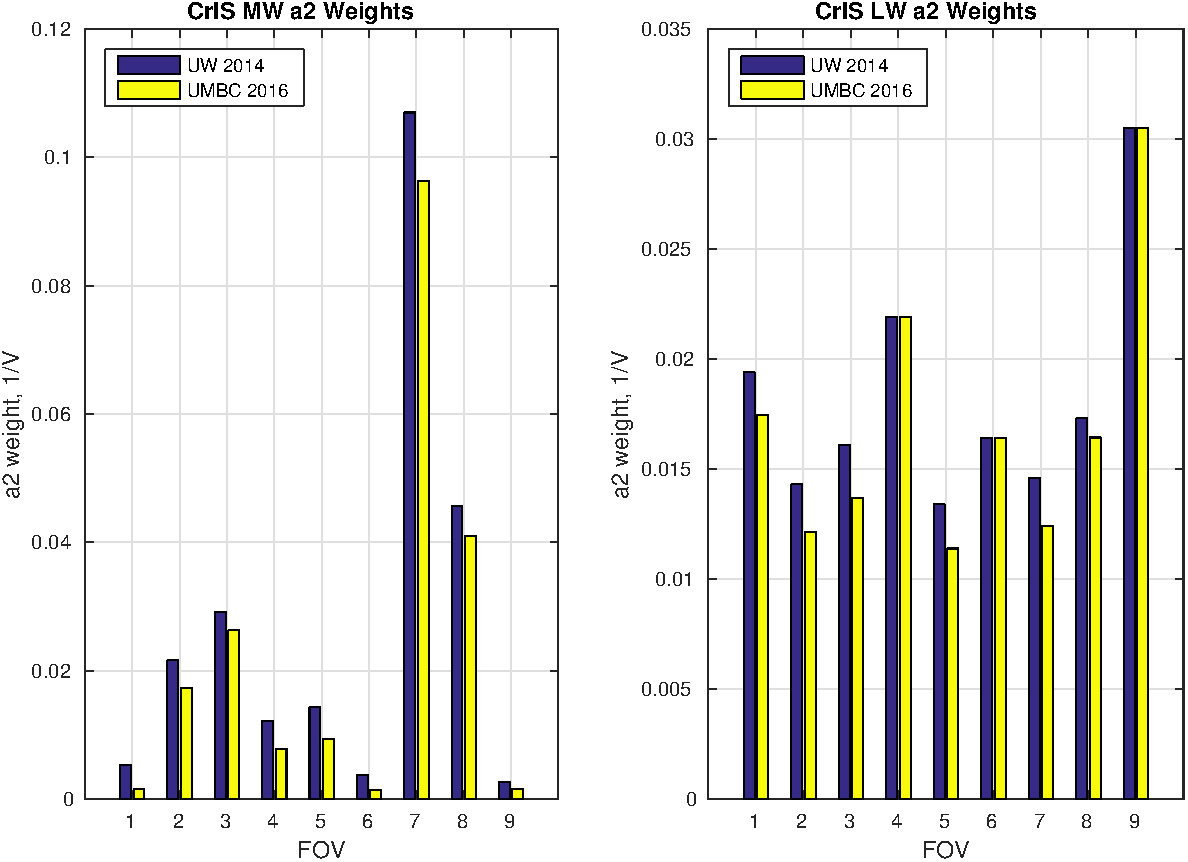
\includegraphics[scale=0.5]{figures/a2_proposed_all.pdf}
\end{center}
\begin{center}
  UW 2014 current and UMBC 2016 proposed a2 values
\end{center}
\end{frame}
%----------- slide --------------------------------------------------%
\begin{frame}
\frametitle{methods}

\begin{itemize}

  \item calibrated radiances are from the UMBC {\ccast} reference
    algorithm, with cosine apodization of extended interferograms,
    periodic sinc wrapping at the sensor grid, and double Fourier
    interpolation to the high res user grid

  \item tests are done with FOR 15 and 16 averaged over 4--6 Dec
    2015

  \item the fitting intervals are 660 to 1060 {\wn} for the LW and
    1250 to 1700 {\wn} for the MW

  \item UW used smaller intervals, 672 to 682 {\wn} for LW and 1585
    to 1600 {\wn} for MW, and averaged low res data over four days

\end{itemize}

\end{frame}
%----------- slide --------------------------------------------------%
\begin{frame}
\frametitle{methods}

\begin{itemize}

  \item the a2 values shown here are expressed as percentages
    (scaling factors) of the 2014 UW a2 values.

  \item brightness temperature averages are taken for separate ccast
    runs with a2 scaling factors ranging from 0 to $1.2$ in steps of
    $0.05$.

  \item these are used to build a 3-D table of mean brightness temp
    spectra by FOV by a2 scaling factor

  \item residuals are the {\rms} average of the difference of
    brightness temperature spectra over the fitting intervals

  \item for a particular FOV, a2 value, and fitting interval we can
    then find a2 values to minimize the residual over the fitting
    interval for all other FOVs

\end{itemize}

\end{frame}
%----------- slide --------------------------------------------------%
\begin{frame}
\frametitle{a2 fitting algorithm}

\begin{itemize}

  \item select the two most linear FOVs, and for each choose an a2
    scaling factor to minimize the sum of all residuals.  For the MW
    this gives a scaling factor of 0.6 for FOV 9 and 0.4 for FOV 6

  \item get the a2 scaling factors for the remaining FOVs at the
    minima of residuals as a function of a2 factors

  \item check that the a2 factors we get from the two most linear
    FOVs agree

  \item check spectral differences of the most and least linear FOVs
    to verify that the a2 selections look sensible

  \item the following slides show these steps for the {\cris} MW
    band, after first finding a2 scaling factors for FOVs 9 and 6 as
    noted above

\end{itemize}

\end{frame}
%----------- slide --------------------------------------------------%
\begin{frame}
\frametitle{MW FOV 9 residuals}
\begin{center}
  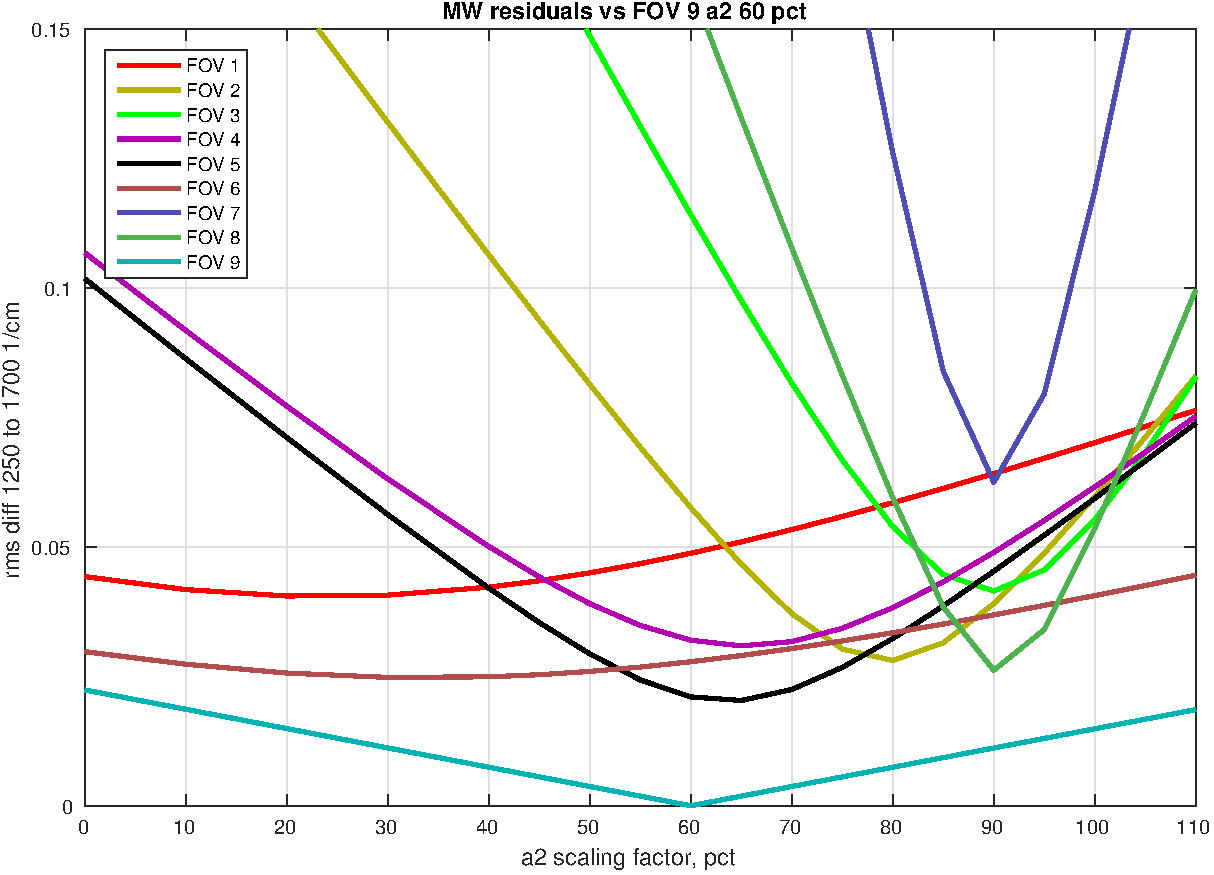
\includegraphics[scale=0.5]{figures/MW_resids_FOV_9_a2_60.pdf}
\end{center}
\begin{center}
  MW fitting residuals for FOV 9 with an a2 scaling factor of 60 pct
\end{center}
\end{frame}
%----------- slide --------------------------------------------------%
\begin{frame}
\frametitle{MW FOV 6 residuals}
\begin{center}
  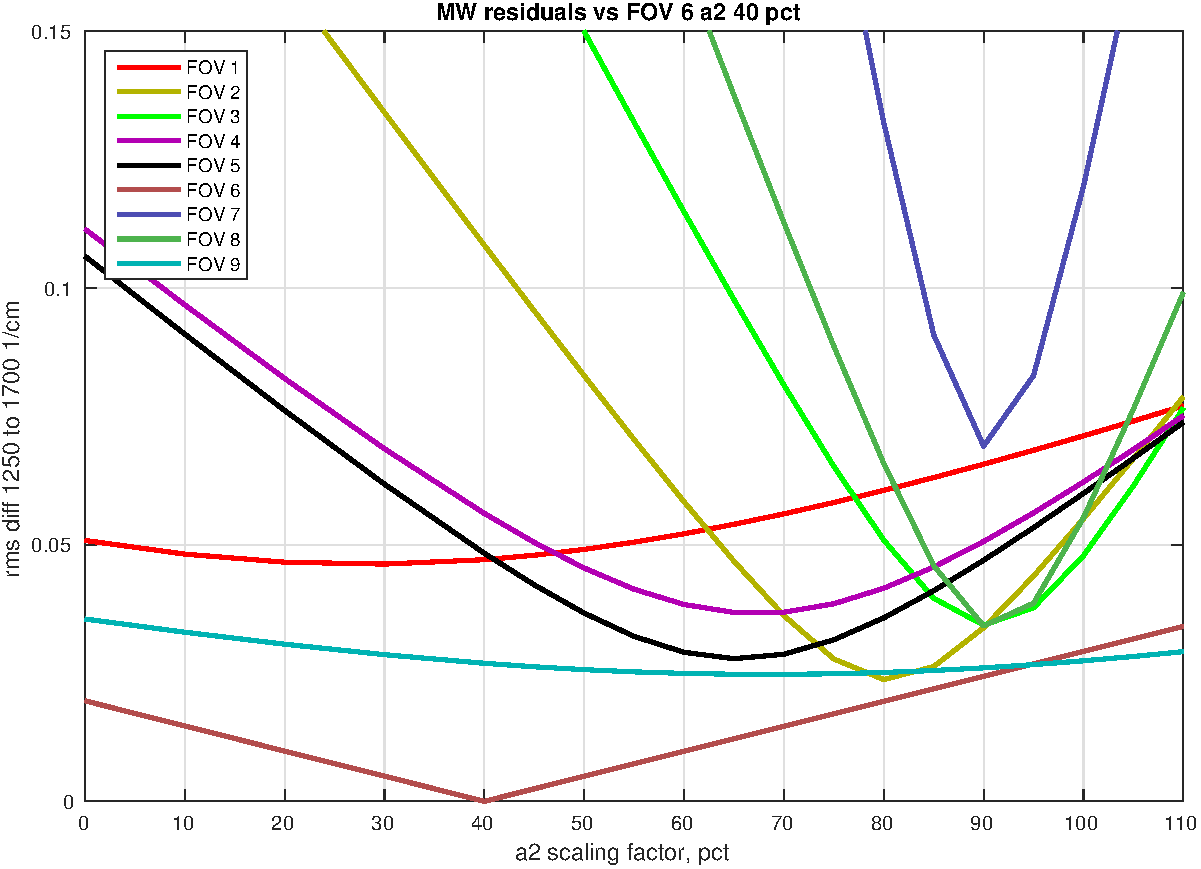
\includegraphics[scale=0.5]{figures/MW_resids_FOV_6_a2_40.pdf}
\end{center}
\begin{center}
  MW fitting residuals for FOV 6 with an a2 scaling factor of 40 pct
\end{center}
\end{frame}
%----------- slide --------------------------------------------------%
\begin{frame}
\frametitle{MW FOV 7 minus FOV 9}
\begin{center}
  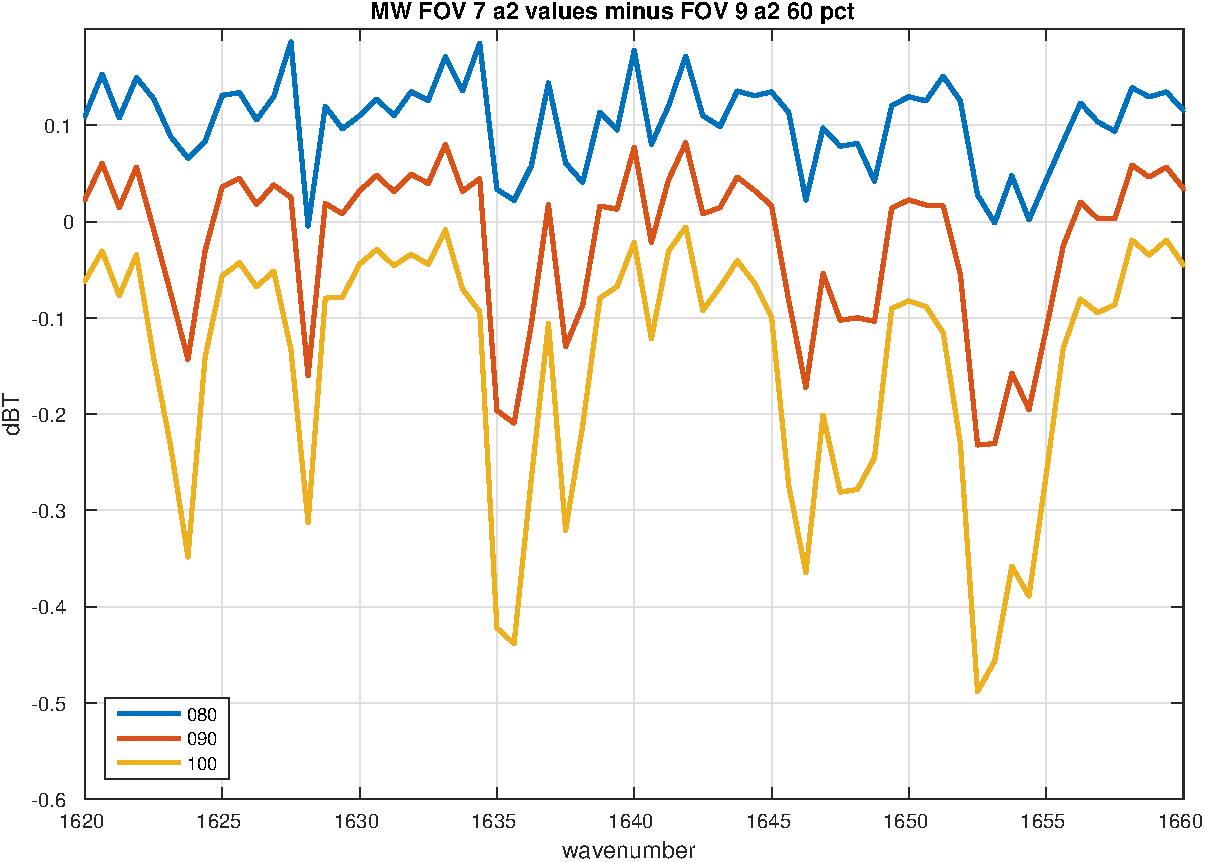
\includegraphics[scale=0.5]{figures/MW_FOV_7_minus_9_a2_60.pdf}
\end{center}  
\begin{center}
  detail of FOV 7 minus FOV 9 spectral difference
\end{center}
\end{frame}
%----------- slide --------------------------------------------------%
\begin{frame}
\frametitle{MW FOV 7 minus FOV 6}
\begin{center}
  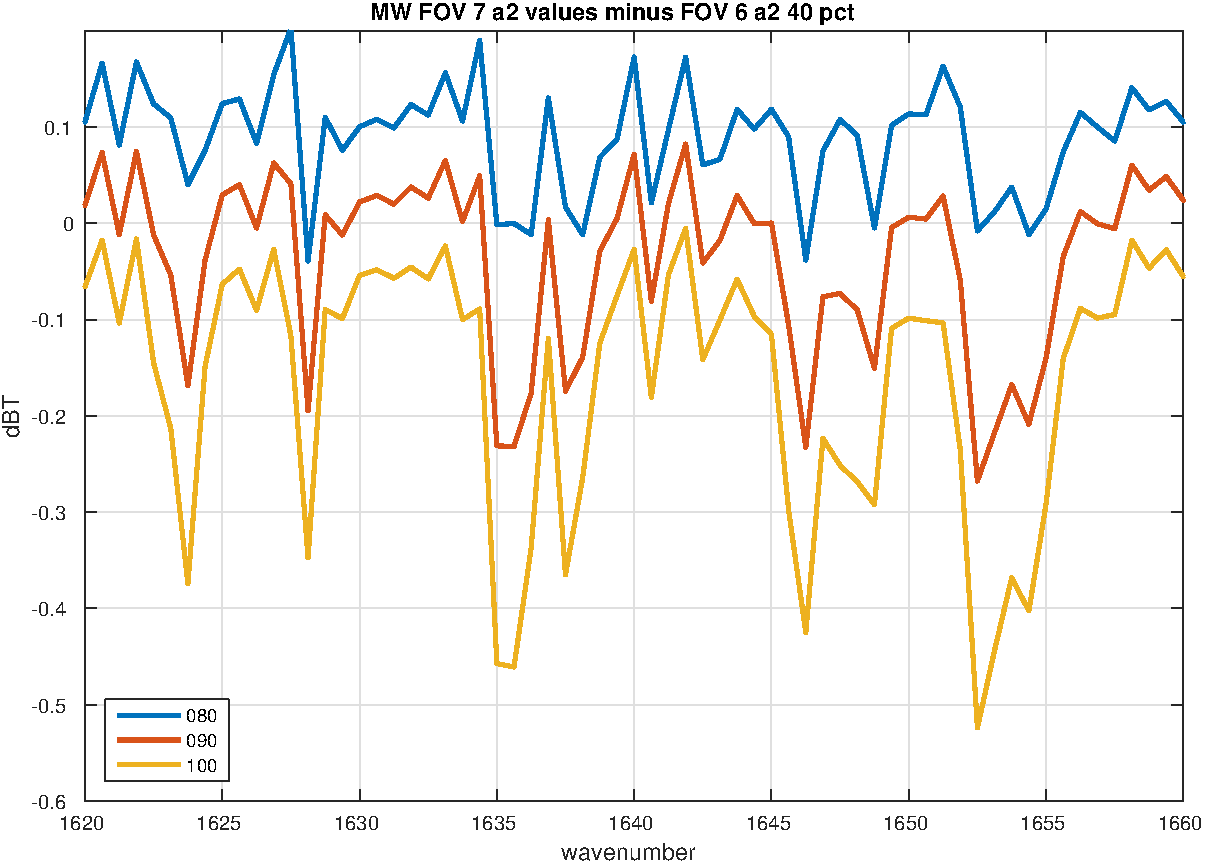
\includegraphics[scale=0.5]{figures/MW_FOV_7_minus_6_a2_40.pdf}
\end{center}
\begin{center}
  detail of FOV 7 minus FOV 6 spectral difference
\end{center}
\end{frame}
%----------- slide --------------------------------------------------%
\begin{frame}
\frametitle{MW FOV 5 relative tests}

\begin{itemize}

  \item to check these results we did {\ccast} runs with the old and
    new a2 values

  \item the following slides show MW FOV 5 relative differences for
    the same 3--day period, using the {\ccast} reference algorithm
    for both the UW 2014 and UMBC 2016 a2 values

  \item we see significant improvements for FOV 7, the least linear,
    and FOVs 9 and 6, the most linear MW FOVs

  \item FOV 2 is slightly improved, FOV 1 slightly worse, and in
    general any changes for the remaining FOVs are small and
    ambiguous

\end{itemize}

\end{frame}
%----------- slide --------------------------------------------------%
\begin{frame}
\frametitle{MW FOV 5 relative tests}
\begin{center}
  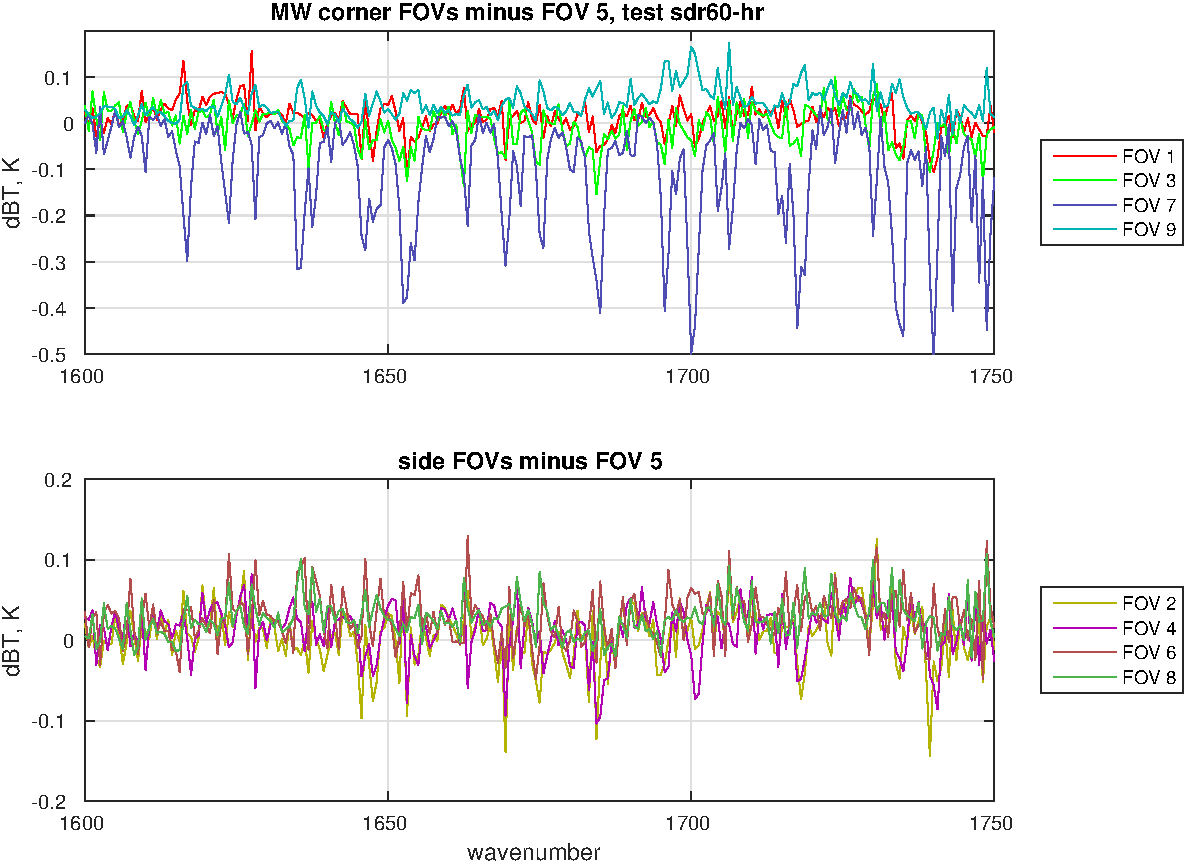
\includegraphics[scale=0.5]{figures/MW_FOV_5_rel_sdr60.pdf}
\end{center}
\begin{center}
  MW FOV 5 relative differences for the UW 2014 a2 values
\end{center}
\end{frame}
%----------- slide --------------------------------------------------%
\begin{frame}
\frametitle{MW FOV 5 relative tests}
\begin{center}
  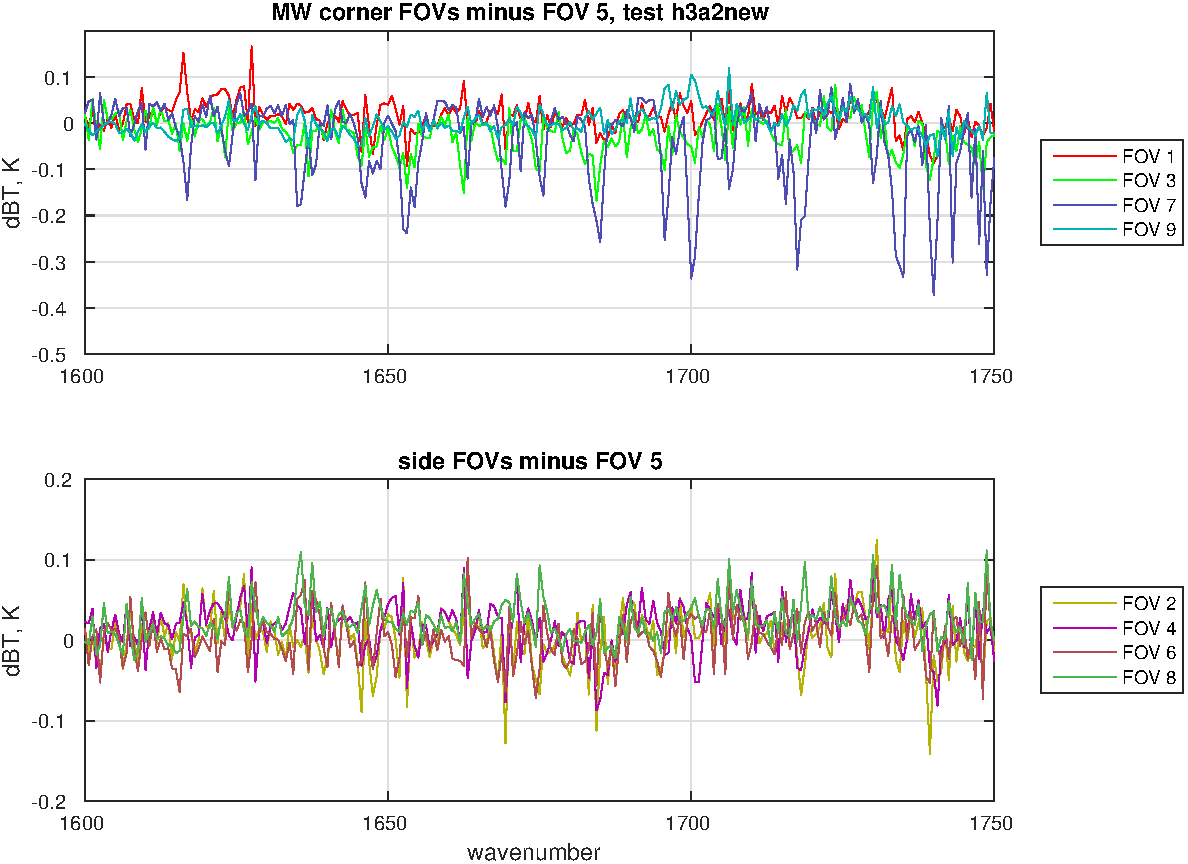
\includegraphics[scale=0.5]{figures/MW_FOV_5_rel_a2new.pdf}
\end{center}
\begin{center}
  MW FOV 5 relative differences for the UMBC 2016 a2 values
\end{center}
\end{frame}
%----------- slide --------------------------------------------------%
\begin{frame}
\frametitle{MW UMBC minus UW a2}
\begin{center}
  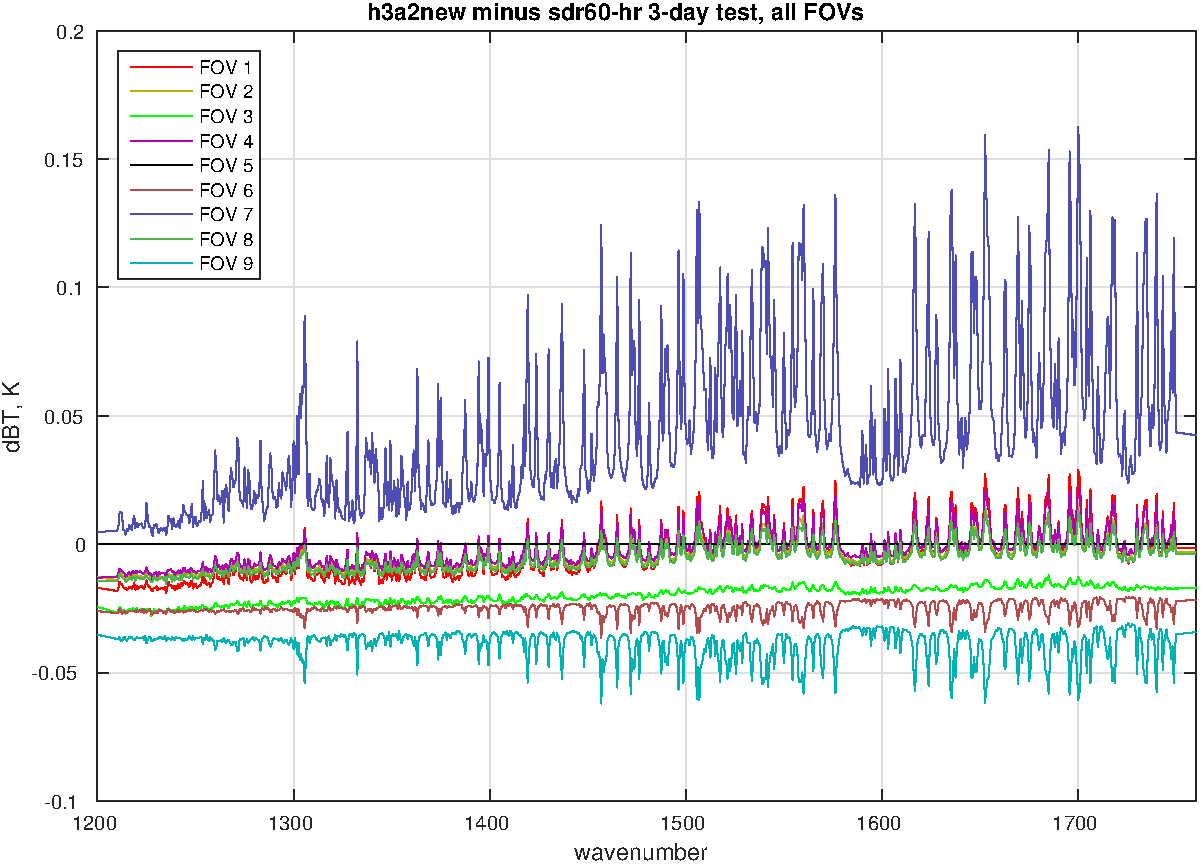
\includegraphics[scale=0.5]{figures/MW_a2new_minus_sdr60.pdf}
\end{center}
\begin{center}
  MW spectral difference for UMBC 2016 and UW 2014 a2 values
\end{center}
\end{frame}
%----------- slide --------------------------------------------------%
\begin{frame}
\frametitle{LW a2 fitting}

\begin{itemize}

  \item the steps above were repeated for the LW band

  \item we start with the two most linear FOVs and find a2 scaling
    factors to minimize the sum of all residuals.  For the LW this
    was 85 pct for FOVs 5 and 2.

  \item residual minima are more closely grouped and the a2 scaling
    factors are closer to 100 pct (the UW values) for the LW, in
    contrast with the MW band

  \item the spectral differences of the most and least linear FOVs
    support the updated a2 selections

  \item however the validation tests show no significant improvement

\end{itemize}

\end{frame}
%----------- slide --------------------------------------------------%
\begin{frame}
\frametitle{LW FOV 5 residuals}
\begin{center}
  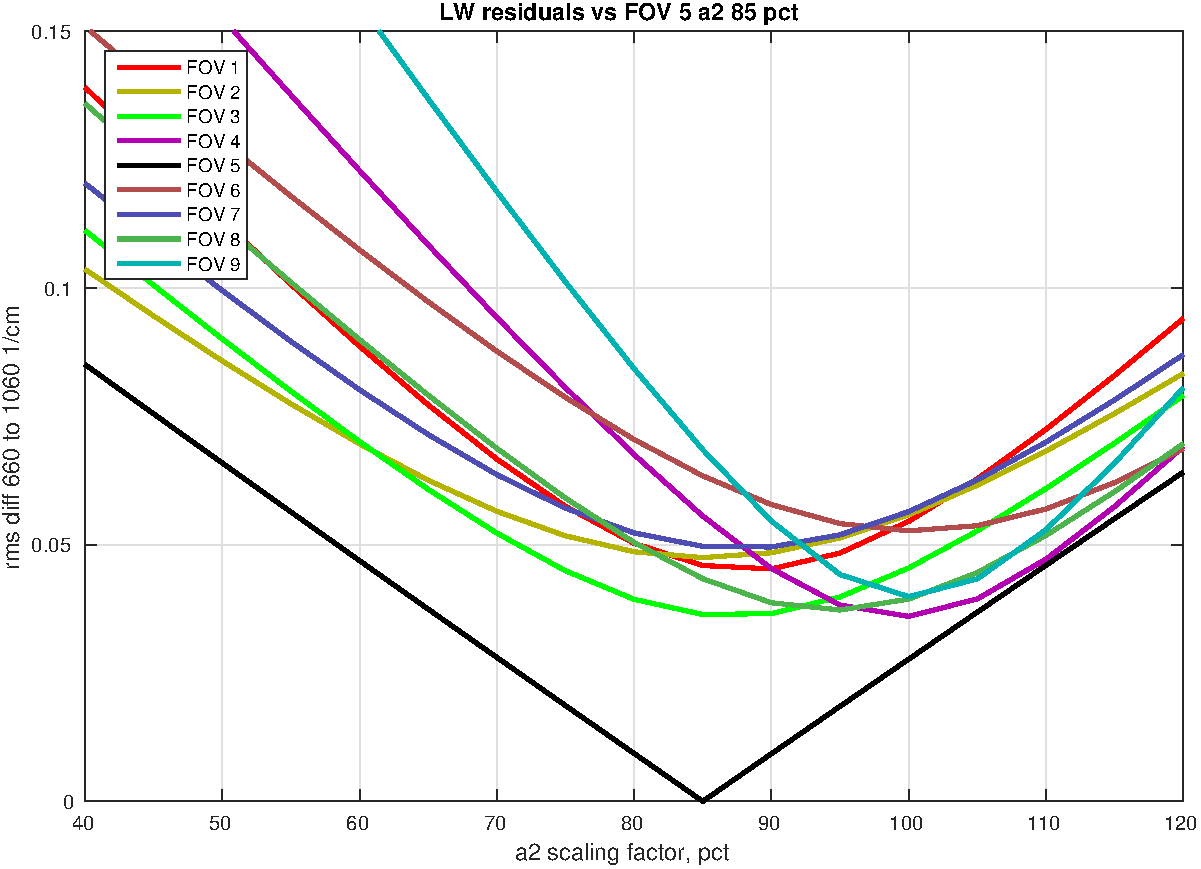
\includegraphics[scale=0.5]{figures/LW_resids_FOV_5_a2_85.pdf}
\end{center}
\begin{center}
  LW fitting residuals for FOV 5 with an a2 scaling factor of 85 pct
\end{center}
\end{frame}
%----------- slide --------------------------------------------------%
\begin{frame}
\frametitle{LW FOV 2 residuals}
\begin{center}
  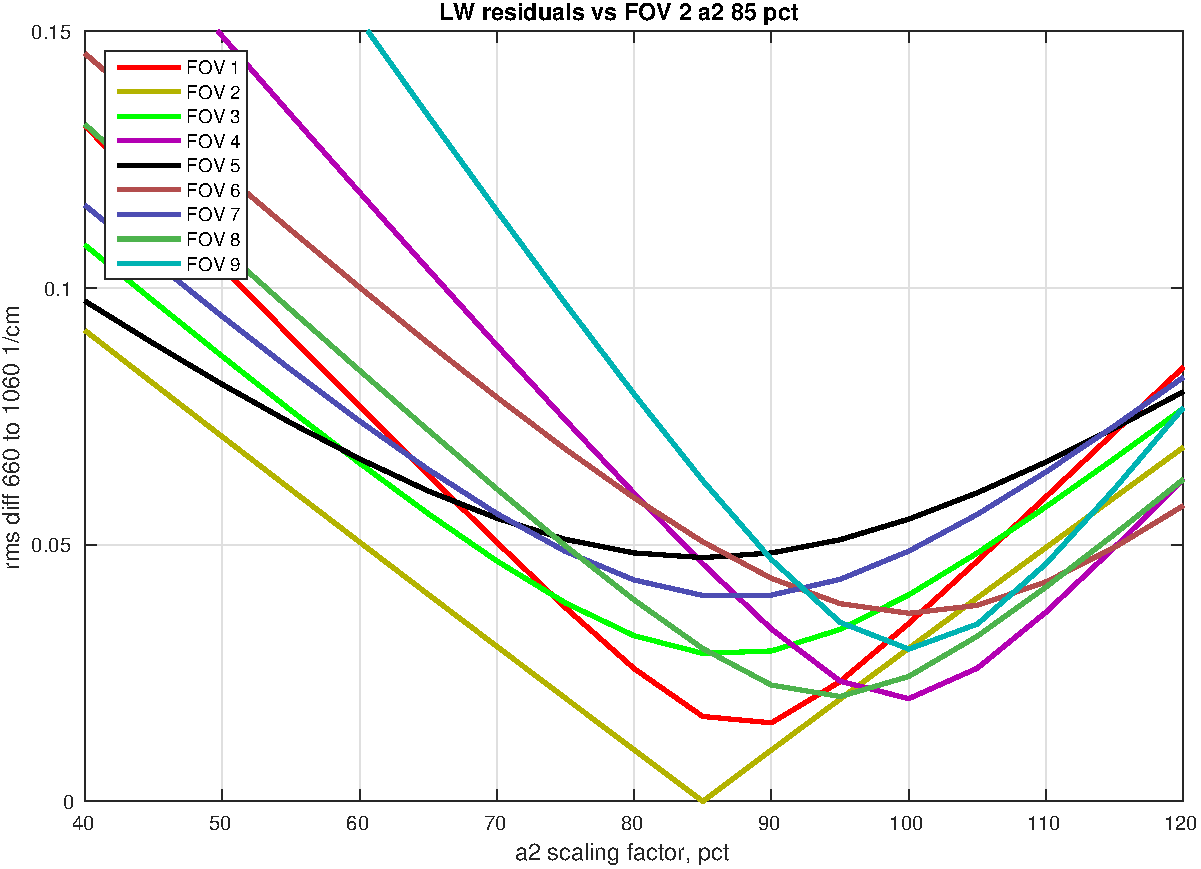
\includegraphics[scale=0.5]{figures/LW_resids_FOV_2_a2_85.pdf}
\end{center}
\begin{center}
  LW fitting residuals for FOV 2 with an a2 scaling factor of 85 pct
\end{center}
\end{frame}
%----------- slide --------------------------------------------------%
\begin{frame}
\frametitle{LW FOV 9 minus FOV 5}
\begin{center}
  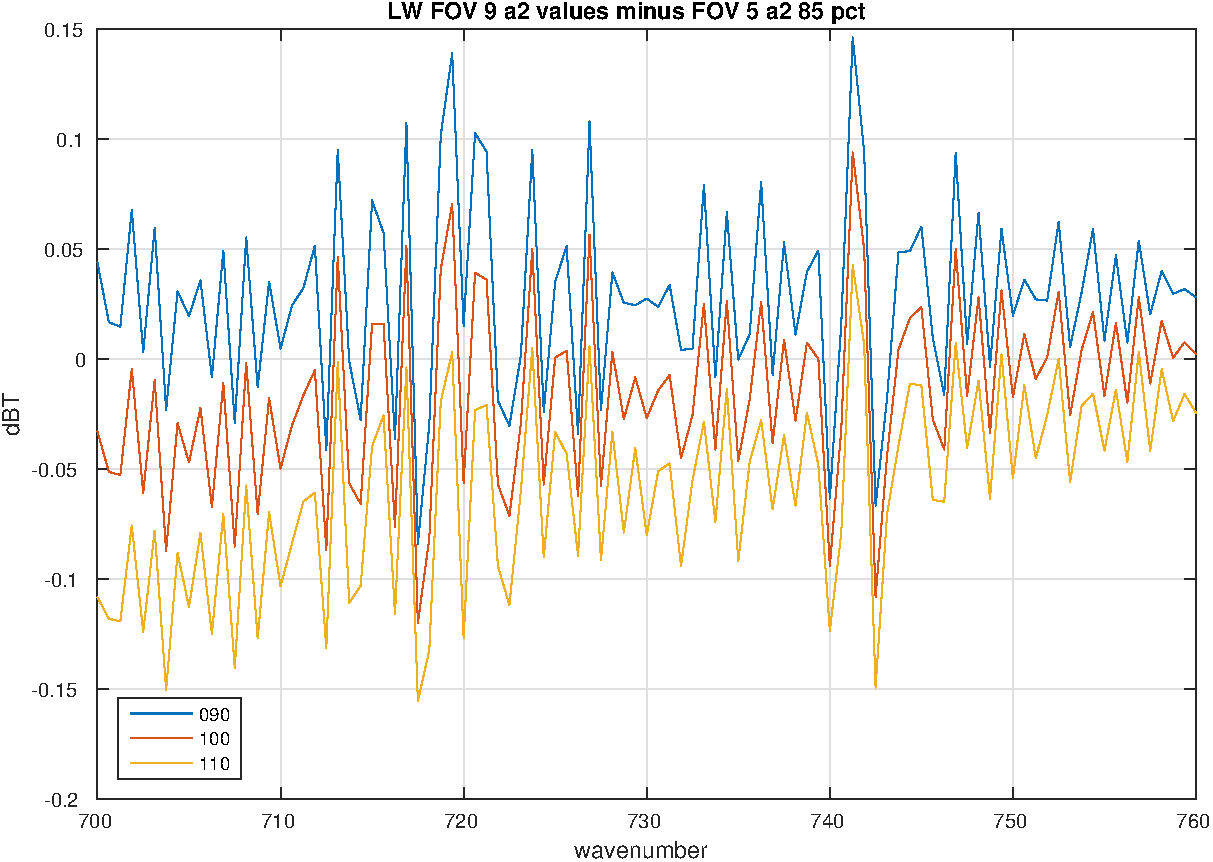
\includegraphics[scale=0.5]{figures/LW_FOV_9_minus_5_a2_85.pdf}
\end{center}  
\begin{center}
  detail of FOV 9 minus FOV 5 spectral difference
\end{center}
\end{frame}
%----------- slide --------------------------------------------------%
\begin{frame}
\frametitle{LW FOV 9 minus FOV 2}
\begin{center}
  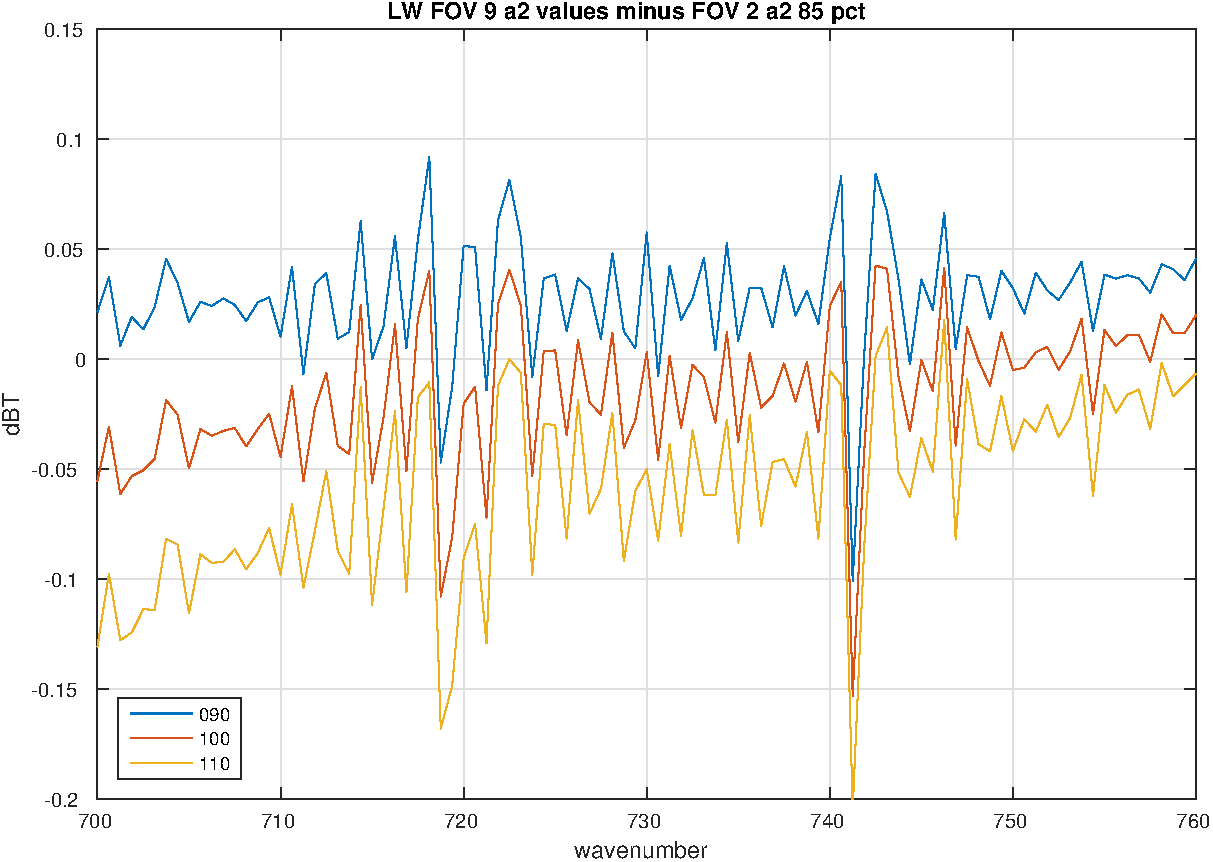
\includegraphics[scale=0.5]{figures/LW_FOV_9_minus_2_a2_85.pdf}
\end{center}  
\begin{center}
  detail of FOV 9 minus FOV 2 spectral difference
\end{center}
\end{frame}
%----------- slide --------------------------------------------------%
\begin{frame}
\frametitle{LW FOV 5 relative tests}
\begin{center}
  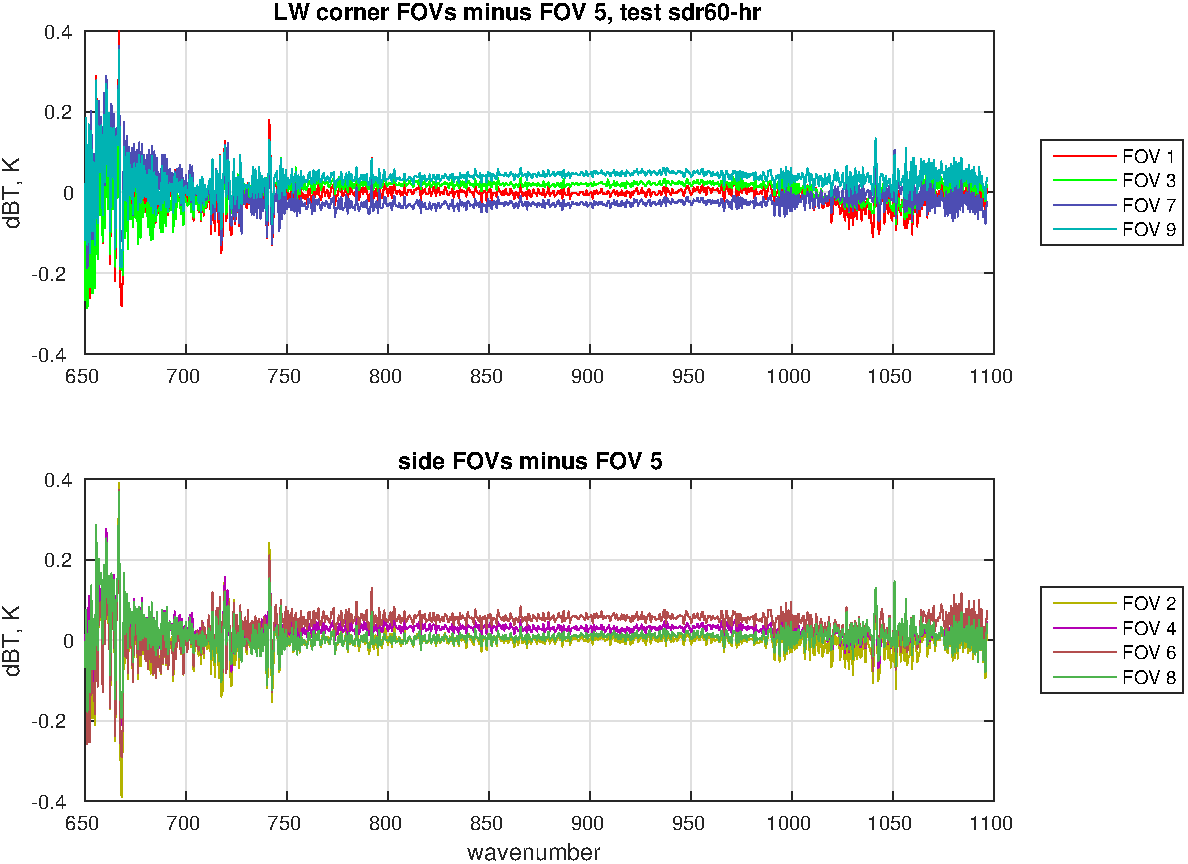
\includegraphics[scale=0.5]{figures/LW_FOV_5_rel_sdr60.pdf}
\end{center}
\begin{center}
  LW FOV 5 relative differences for the UW 2014 a2 values
\end{center}
\end{frame}
%----------- slide --------------------------------------------------%
\begin{frame}
\frametitle{LW FOV 5 relative tests}
\begin{center}
  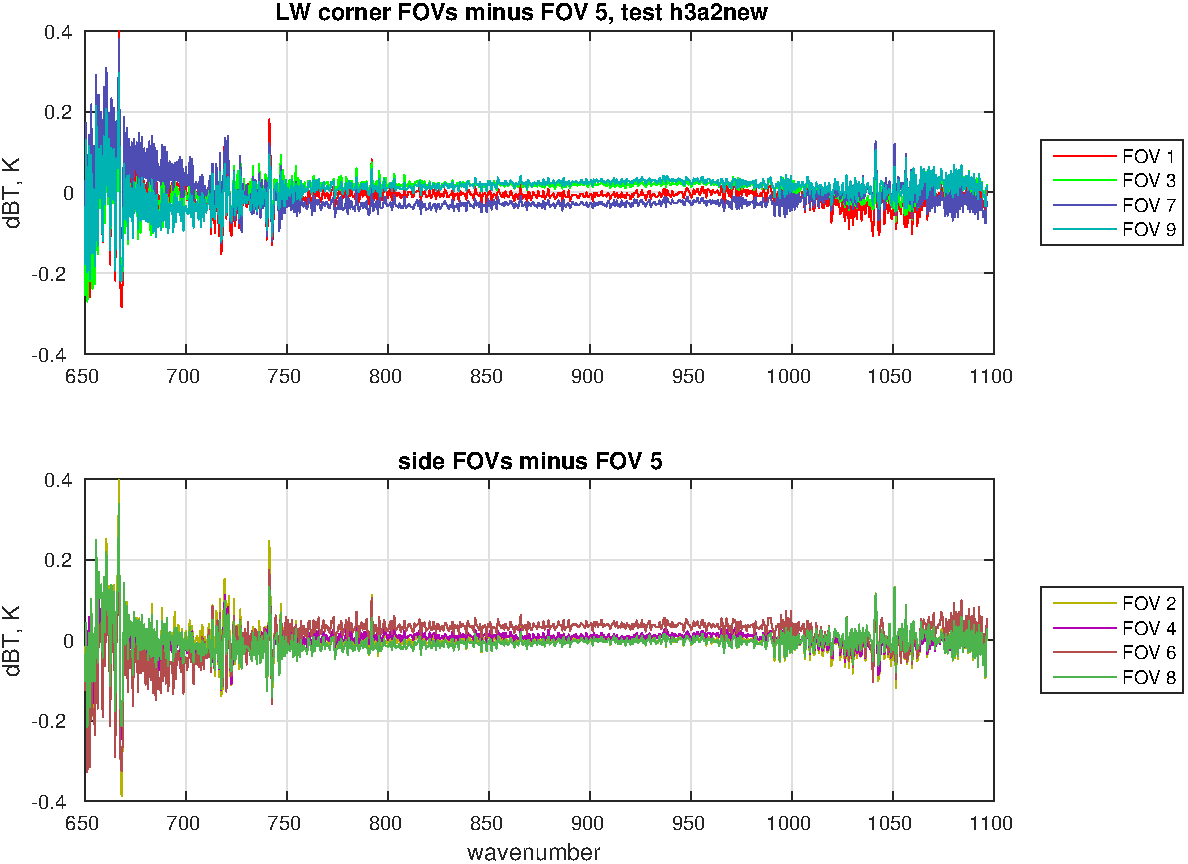
\includegraphics[scale=0.5]{figures/LW_FOV_5_rel_a2new.pdf}
\end{center}
\begin{center}
  LW FOV 5 relative differences for the UMBC 2016 a2 values
\end{center}
\end{frame}
%----------- slide --------------------------------------------------%
\begin{frame}
\frametitle{LW FOV 5 relative tests}
\begin{center}
  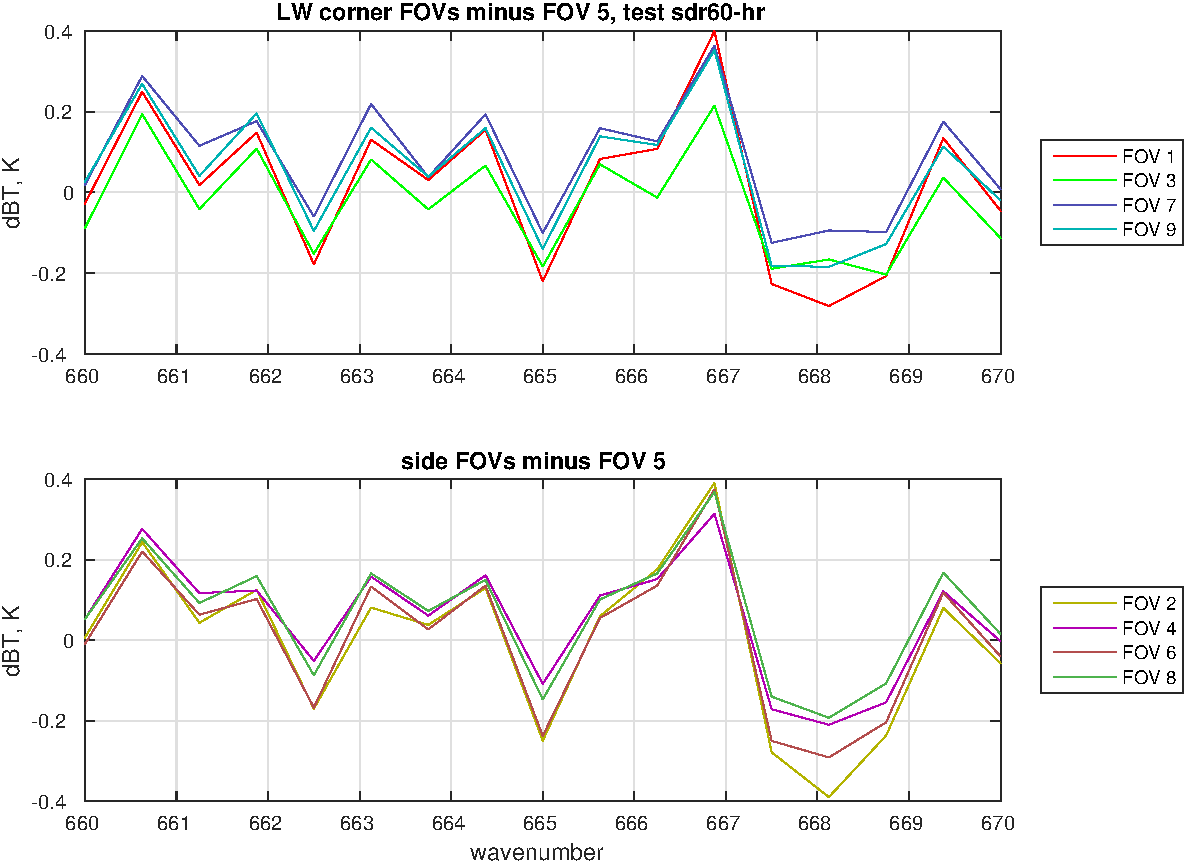
\includegraphics[scale=0.5]{figures/LW_rel_zoom1_sdr60.pdf}
\end{center}
\begin{center}
  LW FOV 5 relative differences for the UW 2014 a2 values, detail
\end{center}
\end{frame}
%----------- slide --------------------------------------------------%
\begin{frame}
\frametitle{LW FOV 5 relative tests}
\begin{center}
  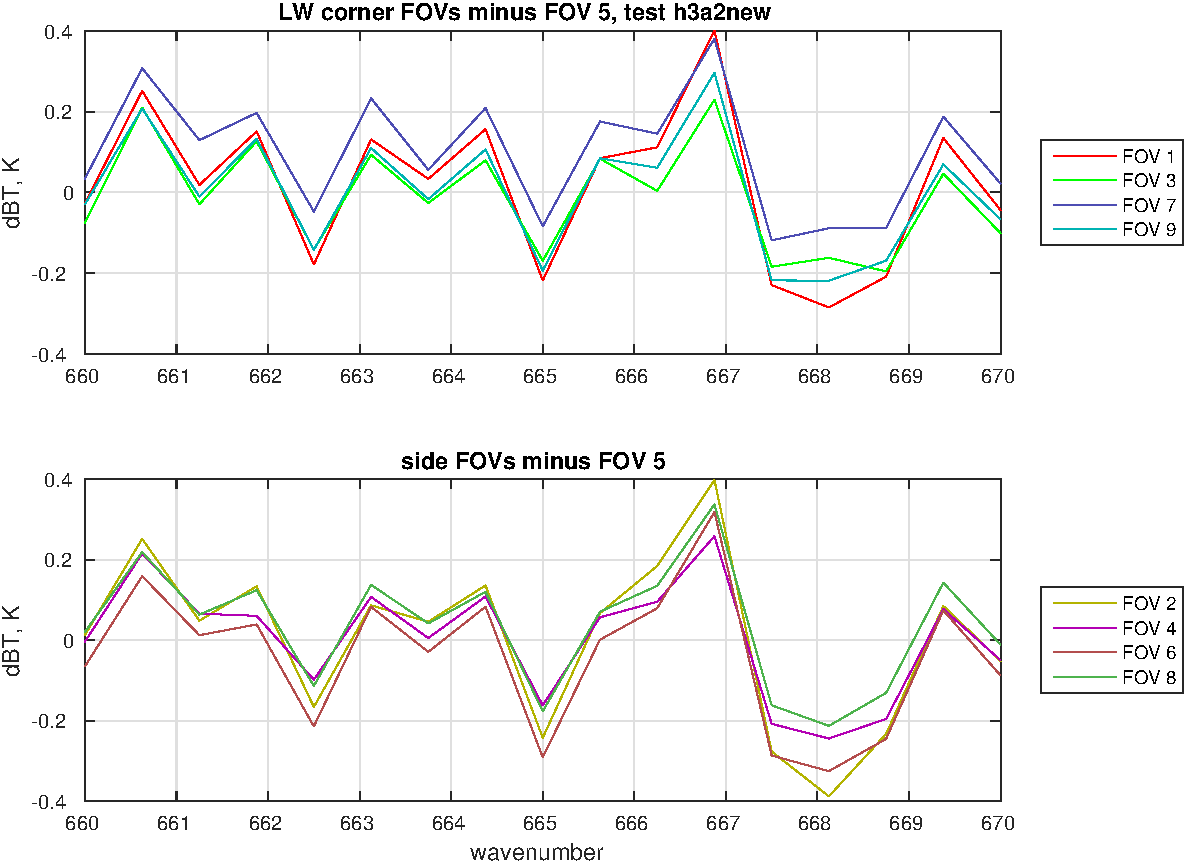
\includegraphics[scale=0.5]{figures/LW_rel_zoom1_a2new.pdf}
\end{center}
\begin{center}
  LW FOV 5 relative differences for the UMBC 2016 a2 values, detail
\end{center}
\end{frame}
%----------- slide --------------------------------------------------%
\begin{frame}
\frametitle{LW FOV 5 relative tests}
\begin{center}
  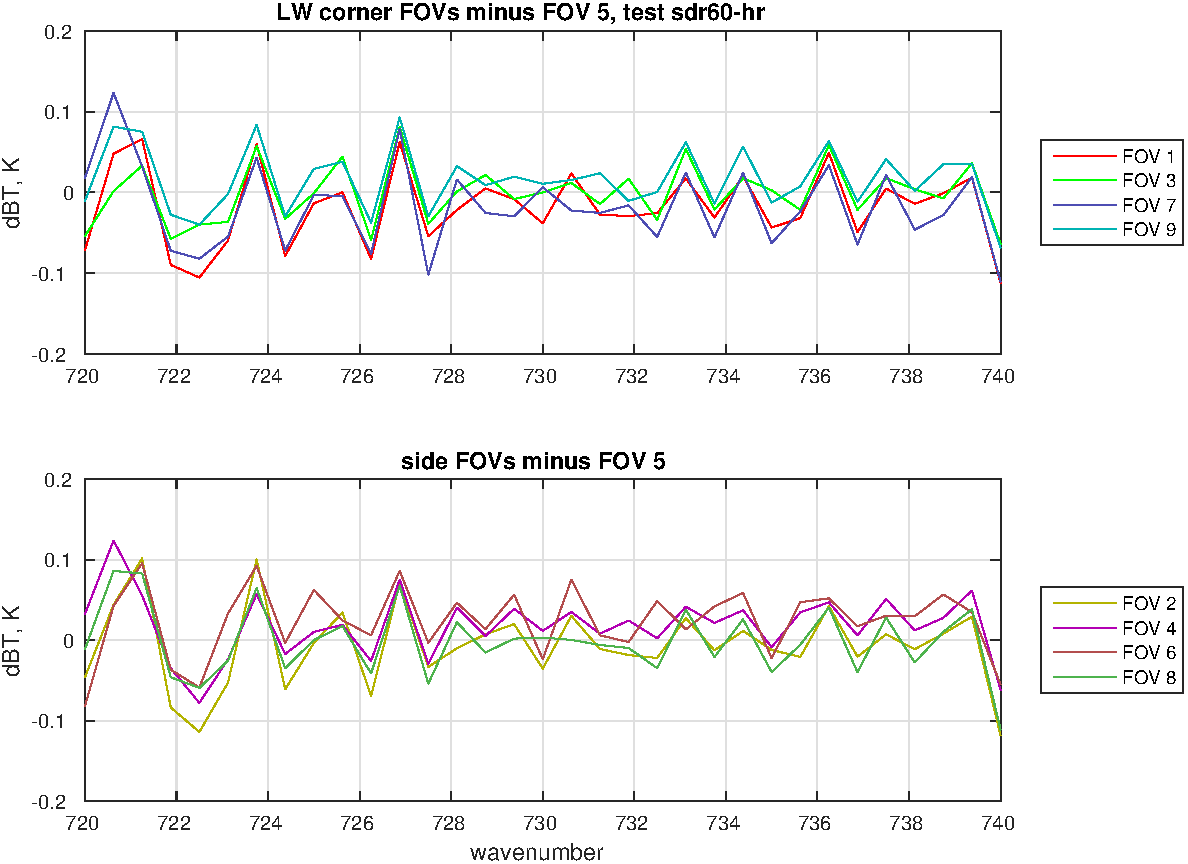
\includegraphics[scale=0.5]{figures/LW_rel_zoom2_sdr60.pdf}
\end{center}
\begin{center}
  LW FOV 5 relative differences for the UW 2014 a2 values, detail
\end{center}
\end{frame}
%----------- slide --------------------------------------------------%
\begin{frame}
\frametitle{LW FOV 5 relative tests}
\begin{center}
  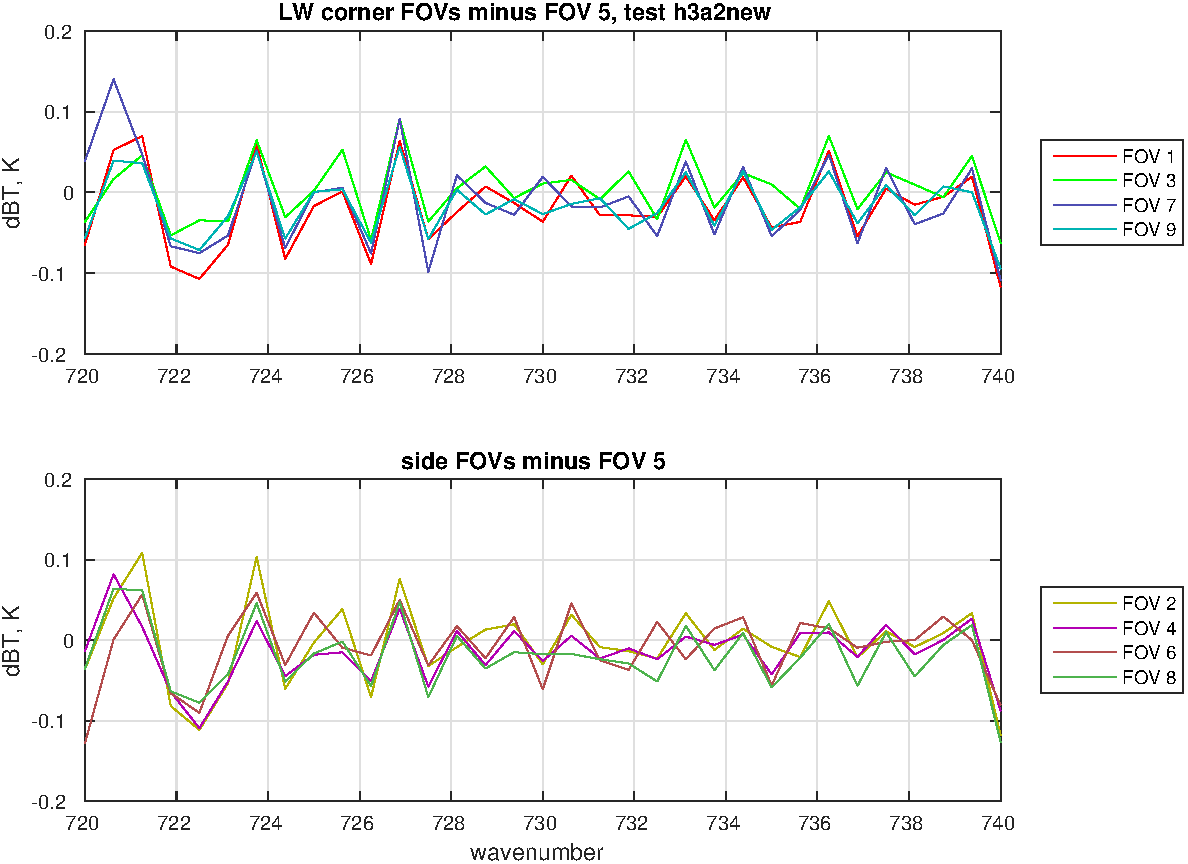
\includegraphics[scale=0.5]{figures/LW_rel_zoom2_a2new.pdf}
\end{center}
\begin{center}
  LW FOV 5 relative differences for the UMBC 2016 a2 values, detail
\end{center}
\end{frame}
%----------- slide --------------------------------------------------%
\begin{frame}
\frametitle{conclusions}

\begin{itemize}

  \item the MW improvement is significant

  \item the resolution of the FOV 5 relative tests may not be
    sufficient to validate the smaller LW a2 changes

  \item the differences in UW and UMBC a2 values are not due just to
    the different fitting intervals---the UMBC algorithm with the UW
    interval gives results that are closer to the UMBC than the UW
    values

  \item if we start the LW fitting with FOVs 5 and 2 at 100 pct
    rather than 85 pct (that is, with the UW a2 values) the other
    scaling factors also increase by 10 or 15 pct and the fitting
    residuals become slightly larger

\end{itemize}

\end{frame}
% %----------- slide --------------------------------------------------%
% \begin{frame}
% \frametitle{ccast calibration equation}
% 
% \[\rES = F \cdot \rIT \cdot f \cdot \SA^{-1}\cdot f \cdot 
%          \frac{\ES - \SPmean}{\ITmean - \SPmean} \]
% 
% \begin{itemize}
%   \item $\rES$ is calibrated earth-scene radiance at the user grid
%   \item $F$ is Fourier interpolation from sensor to user grid
%   \item $\rIT$ is expected ICT radiance at the sensor grid
%   \item $f$ is a raised-cosine bandpass filter with wings at or just
%     inside instrument responsivity
%   \item $\SA$ is from a periodic sinc ILS wrapping at the sensor
%     grid
%   \item $\ES$, $\ITmean$ and $\SPmean$ are corrected for
%     nonlinearity
%   \item $\ITmean$ and $\SPmean$ are averages over 9 scans
% \end{itemize}
% 
% \end{frame}
%----------- slide --------------------------------------------------%
\end{document}

